% Worksheet W3 – Dimensions of time (2 pages), lesson with the website
% Übersetzen: latexmk -xelatex ws-w3-dimensions-of-time.tex
% ============================================================
% ab-vorlage.tex – gemeinsame Vorlage der Arbeitsblätter
% englisch/12/w-seminar-time/arbeitsblaetter/  (W-Seminar "Time")
% Übersetzen mit:  latexmk -xelatex <datei>.tex   (oder zweimal xelatex)
% Gestaltung wie englisch/13/questions-on-the-text/arbeitsblaetter/ab-vorlage.tex,
% Antwortplatz-Makros (8-mm-Linien) wie informatik/10/java/arbeitsblaetter/ab-vorlage.tex
% Schriften: Carlito (Fließtext), Poppins (Überschriften)
% ============================================================
\documentclass[10pt,a4paper]{article}
\usepackage[a4paper,top=12mm,bottom=13mm,left=14mm,right=14mm,headsep=4mm,headheight=12pt,footskip=7mm]{geometry}
\usepackage{fontspec}
\setmainfont{Carlito}
\newfontfamily\headfont{Poppins}[UprightFont=* Medium, BoldFont=* Medium]
\newfontfamily\headlight{Poppins Light}
\usepackage{xcolor}
\definecolor{prim}{HTML}{2563EB}
\definecolor{primdark}{HTML}{1E3A8A}
\definecolor{sec}{HTML}{7C3AED}
\definecolor{dusk}{HTML}{171A3F}
\definecolor{brass}{HTML}{D9AB2F}
\definecolor{primtint}{HTML}{EFF6FF}
\definecolor{sectint}{HTML}{F5F3FF}
\definecolor{ink}{HTML}{1E293B}
\definecolor{muted}{HTML}{64748B}
\definecolor{rule}{HTML}{CBD5E1}
\definecolor{good}{HTML}{059669}
\definecolor{goodtint}{HTML}{ECFDF5}
\definecolor{warn}{HTML}{B45309}
\definecolor{warntint}{HTML}{FFFBEB}
\definecolor{bad}{HTML}{B91C1C}
\definecolor{badtint}{HTML}{FEF2F2}
% Farben der Zeit-Dimensionen (wie auf der Website)
\definecolor{dlit}{HTML}{B83280}
\definecolor{dphys}{HTML}{2563EB}
\definecolor{dcs}{HTML}{0F8F84}
\definecolor{dpsy}{HTML}{C26A06}
\definecolor{dlang}{HTML}{7C3AED}
\definecolor{dbey}{HTML}{4B5563}
\color{ink}
\usepackage[most]{tcolorbox}
\usepackage{tikz}
\usetikzlibrary{positioning,calc,arrows.meta,shapes.misc}
\usepackage{enumitem}
\setlist{nosep,leftmargin=1.1em,topsep=1pt}
\setlist[itemize]{label=\textcolor{prim}{\small\textbullet}}
\usepackage{tabularx,array,booktabs,colortbl}
\usepackage{multicol}
\usepackage{fancyhdr}
\usepackage{lastpage}
\usepackage{amssymb}
\usepackage{qrcode}
\usepackage{microtype}
\setlength{\parindent}{0pt}
\setlength{\parskip}{0pt}
\linespread{1.02}

% ---------- Kopf- und Fußzeile ----------
\newcommand{\wskopf}{W-Seminar English · Time · Year 12}
\pagestyle{fancy}
\fancyhf{}
\renewcommand{\headrulewidth}{0pt}
\fancyhead[L]{\footnotesize\headlight\textcolor{muted}{\wskopf}}
\fancyhead[R]{\ifnum\value{page}=1\footnotesize\headlight\textcolor{muted}{Name: \rule{38mm}{0.3pt}\quad Date: \rule{18mm}{0.3pt}}\fi}
\fancyfoot[L]{\scriptsize\textcolor{muted}{edu-mrh.de/englisch/12/w-seminar-time}}
\fancyfoot[R]{\scriptsize\textcolor{muted}{\thepage\,/\,\pageref*{LastPage}}}

% ---------- Titel ----------
% \wstitel{Kürzel}{Titel}{Untertitel}
\newcommand{\wstitel}[3]{%
  \begin{tcolorbox}[enhanced,colback=dusk,colframe=dusk,arc=2mm,boxrule=0pt,
     left=4mm,right=4mm,top=2.2mm,bottom=2.2mm,
     interior style={left color=dusk,right color=primdark}]
    \color{white}{\headlight\footnotesize #1}\\[0.3mm]
    {\headfont\LARGE #2}\\[0.6mm]
    {\small #3}
  \end{tcolorbox}\vspace{1mm}}

% ---------- Boxen ----------
% \begin{wsbox}[Optionen]{Nummer}{Überschrift} ... \end{wsbox}
\newtcolorbox{wsbox}[3][]{enhanced,breakable,colback=white,colframe=rule,boxrule=0.5pt,arc=1.5mm,
  left=2.5mm,right=2.5mm,top=1.3mm,bottom=1.3mm,
  title={\headfont\normalsize\textcolor{white}{\colorbox{prim}{\,#2\,}}\;\textcolor{ink}{#3}},
  coltitle=ink,colbacktitle=white,attach title to upper={\par\vspace{0.6mm}},before skip=1.4mm,after skip=1.4mm,#1}
\newtcolorbox{tintbox}[1][]{enhanced,colback=primtint,colframe=primtint,boxrule=0pt,arc=1.2mm,
  left=2mm,right=2mm,top=1.2mm,bottom=1.2mm,#1}
\newtcolorbox{secbox}[1][]{enhanced,colback=sectint,colframe=sectint,boxrule=0pt,arc=1.2mm,
  left=2mm,right=2mm,top=1.2mm,bottom=1.2mm,#1}
\newtcolorbox{goodbox}[1][]{enhanced,colback=goodtint,colframe=goodtint,boxrule=0pt,arc=1.2mm,
  left=2mm,right=2mm,top=1.2mm,bottom=1.2mm,#1}
\newtcolorbox{warnbox}[1][]{enhanced,colback=warntint,colframe=warntint,boxrule=0pt,arc=1.2mm,
  left=2mm,right=2mm,top=1.2mm,bottom=1.2mm,#1}
\newtcolorbox{badbox}[1][]{enhanced,colback=badtint,colframe=badtint,boxrule=0pt,arc=1.2mm,
  left=2mm,right=2mm,top=1.2mm,bottom=1.2mm,#1}

\newcommand{\kl}[1]{{\headfont\small\textcolor{prim}{#1}}}      % kleine Zwischenüberschrift
\newcommand{\klsec}[1]{{\headfont\small\textcolor{sec}{#1}}}
\newcommand{\klc}[2]{{\headfont\small\textcolor{#1}{#2}}}       % Zwischenüberschrift in Farbe
\newcommand{\plus}{\textcolor{good}{\textbf{+}}\ }
\newcommand{\minus}{\textcolor{bad}{\textbf{–}}\ }
\newcommand{\pfeil}{\textcolor{prim}{$\rightarrow$}\ }
\newcommand{\cb}{\raisebox{-0.2ex}{\textcolor{muted}{$\square$}}\ }   % Ankreuzkästchen

% ---------- Antwortplatz (8 mm, wie informatik/10/java) ----------
\newif\ifloesung
\ifdefined\mitloesung \loesungtrue \else \loesungfalse \fi
\newcommand{\lsgfarbe}{\color{sec}\itshape}
\newlength{\zeilenabstand}\setlength{\zeilenabstand}{8mm}
\tikzset{schreiblinie/.style={draw=black!45,line width=0.35pt}}
% Lücke: \luecke[Breite] / \lsg[Breite]{Text}
\newcommand{\lsg}[2][45mm]{%
  \makebox[#1][l]{\rlap{\raisebox{-0.6ex}{\rule{#1}{0.4pt}}}\ifloesung{\lsgfarbe\small\,#2}\fi}}
\newcommand{\luecke}[1][45mm]{\lsg[#1]{}}
% Lücke bis Zeilenende
\newcommand{\lsgrest}[1]{\leavevmode\unskip\hspace{1.5mm}\ifloesung\rlap{\raisebox{0.8pt}{\lsgfarbe\,#1}}\fi\leaders\hbox{\rule[-0.6ex]{0.5pt}{0.4pt}}\hfill\null\par}
\newcommand{\restzeile}{\lsgrest{}}
\newcommand{\lueckentext}{\linespread{1.5}\selectfont\raggedright}
\newcommand{\schreibzeile}{\rule[-2.8mm]{0pt}{8mm}}
% Schreiblinien: \linien{n} / \lsglinien{n}{Text}; erste Linie eine volle Zeilenhöhe unter der Frage
\newcommand{\lsglinien}[2]{\par\vspace{0.5mm}\noindent\begin{tikzpicture}
  \path (0,0) (\linewidth-0.4pt,-#1\zeilenabstand-1.5mm);
  \foreach \i in {1,...,#1}{\draw[schreiblinie] (0.2pt,-\i\zeilenabstand) -- (\linewidth-0.2pt,-\i\zeilenabstand);}
  \ifloesung\node[overlay,anchor=north west,inner sep=0pt] at (1mm,-\zeilenabstand+1pt+5mm) {\parbox[t]{\linewidth-2mm}{\lsgfarbe\raggedright\setlength{\baselineskip}{\zeilenabstand}\rule{0pt}{5mm}#2}};\fi
  \end{tikzpicture}\par}
\newcommand{\linien}[1]{\lsglinien{#1}{}}

\newcommand{\website}{https://edu-mrh.de/englisch/12/w-seminar-time/w-seminar-time.html}

\begin{document}

\wstitel{Worksheet W3 · W-Seminar “Time”}{Dimensions of time}%
{Time is not one thing. Today you become the expert for one of its dimensions – and look for your own question.}

% ------------------------------------------------------------------ 1
\begin{wsbox}{1}{Warm-up: feel ten seconds}
\begin{minipage}[t]{0.56\linewidth}\vspace{0pt}
Open the website, scroll to \emph{Psychology} and do the experiment: three tries just waiting, three tries counting backwards.\par\vspace{1mm}
\renewcommand{\arraystretch}{1}
{\small
\begin{tabularx}{\linewidth}{@{}l *{3}{>{\centering\arraybackslash}X} >{\centering\arraybackslash}X@{}}
\arrayrulecolor{rule}\toprule
 & \textbf{try 1} & \textbf{try 2} & \textbf{try 3} & \textbf{mean}\\\midrule
\schreibzeile just wait & & & & \\\midrule
\schreibzeile counting & & & & \\\bottomrule
\end{tabularx}}
\end{minipage}\hfill
\begin{minipage}[t]{0.41\linewidth}\vspace{0pt}
\kl{What could explain the difference?}
\linien{2}
\end{minipage}
\end{wsbox}

% ------------------------------------------------------------------ 2
\begin{wsbox}{2}{Before you look: where does time show up?}
{\small Collect everything you associate with time – subjects, situations, films, books, feelings.}\par\vspace{1mm}
\centering
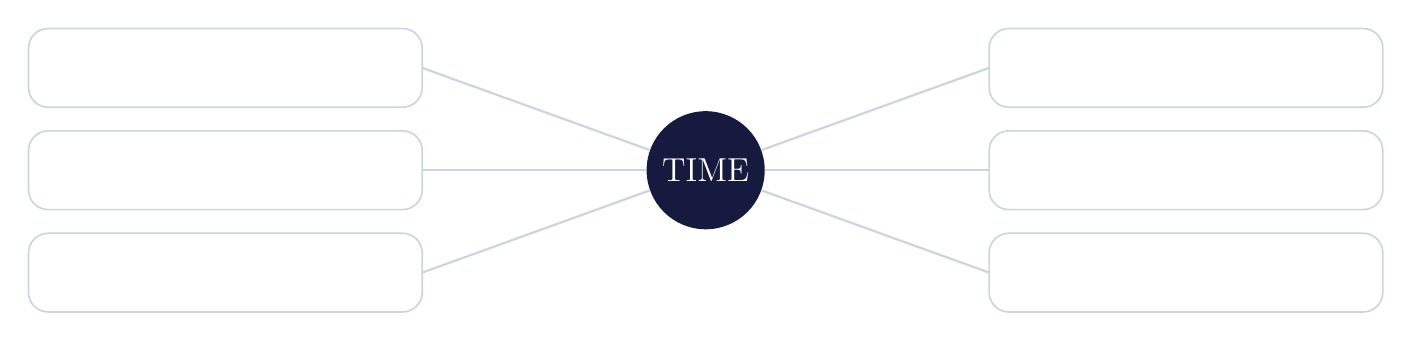
\begin{tikzpicture}[x=1mm,y=1mm]
  \node[circle,fill=dusk,text=white,font=\headfont\large,minimum size=15mm] (t) at (0,0) {TIME};
  \foreach \sx in {-1,1} \foreach \y in {13,0,-13} {
    \draw[rule,line width=0.8pt] (t) -- (\sx*36,\y);
    \draw[rule,fill=white,rounded corners=2.5mm,line width=0.6pt] (\sx*36,\y-5) rectangle (\sx*86,\y+5);
  }
\end{tikzpicture}
\end{wsbox}

% ------------------------------------------------------------------ 3
\begin{wsbox}{3}{Expert group: your dimension}
\begin{minipage}[t]{0.8\linewidth}\vspace{0pt}
\kl{Our dimension}\par\vspace{0.5mm}{\small
\cb\textcolor{dlit}{Literature}\quad \cb\textcolor{dphys}{Physics}\quad \cb\textcolor{dcs}{Computer science}\quad
\cb\textcolor{dpsy}{Psychology}\quad \cb\textcolor{dlang}{Language}\quad \cb\textcolor{dbey}{And beyond}}\par\vspace{1mm}
{\small Explore your section on the website (15 min). Read, try every interactive part, discuss. Then fill in your expert card together.}
\end{minipage}\hfill
\begin{minipage}[t]{0.17\linewidth}\vspace{0pt}\raggedleft
\qrcode[height=19mm]{\website}
\end{minipage}
\par\vspace{1mm}
\kl{The key idea in one or two sentences}
\linien{2}
\kl{The most surprising fact}
\linien{1}
\kl{What we found out with the interactive part}
\linien{2}
\kl{A question that still bothers us}
\linien{1}
\kl{A possible Seminararbeit question – and how we could find out}\enspace{\small\textcolor{muted}{(survey, experiment, text analysis, measurement …)}}
\linien{2}
\end{wsbox}

% ================================================================== page 2
\newpage
% ------------------------------------------------------------------ 4
\begin{wsbox}{4}{Pitch and listen}
{\small Each group pitches its dimension in \textbf{90 seconds}: key idea, wow fact, one question. Listen and take notes.}\par\vspace{1mm}
\renewcommand{\arraystretch}{1}
\begin{tabularx}{\linewidth}{@{}>{\raggedright\arraybackslash}p{31mm} X X@{}}
\arrayrulecolor{rule}\toprule
 & \textbf{key idea} & \textbf{a question I find interesting}\\\midrule
\rule[-7mm]{0pt}{17mm}\klc{dlit}{Literature} & & \\\midrule
\rule[-7mm]{0pt}{17mm}\klc{dphys}{Physics} & & \\\midrule
\rule[-7mm]{0pt}{17mm}\klc{dcs}{Computer science} & & \\\midrule
\rule[-7mm]{0pt}{17mm}\klc{dpsy}{Psychology} & & \\\midrule
\rule[-7mm]{0pt}{17mm}\klc{dlang}{Language} & & \\\midrule
\rule[-7mm]{0pt}{17mm}\klc{dbey}{And beyond} & & \\\bottomrule
\end{tabularx}
\end{wsbox}

% ------------------------------------------------------------------ 5
\begin{wsbox}{5}{Connect two dimensions}
\begin{minipage}[t]{0.42\linewidth}\vspace{0pt}
\begin{tintbox}\small
\textbf{Example:} In Ted Chiang's “Story of Your Life”, learning a new \textcolor{dlang}{language} changes how a character experiences time – and so the \textcolor{dlit}{story} is told in a new tense.
\end{tintbox}
\end{minipage}\hfill
\begin{minipage}[t]{0.55\linewidth}\vspace{0pt}
\kl{Your connection: \luecke[22mm] \,+\, \luecke[22mm]}
\linien{3}
\end{minipage}
\end{wsbox}

% ------------------------------------------------------------------ 6
\begin{wsbox}{6}{Exit ticket}
\begin{lueckentext}
My two favourite dimensions: \luecke[45mm] and \luecke[45mm]\par
\end{lueckentext}
\vspace{0.5mm}
\kl{A question I might research}
\linien{3}
\vspace{1mm}
\kl{How ready do I feel to choose a topic?}\quad
{\small not at all}\enspace
\foreach \n in {1,...,5}{\tikz[baseline=-0.6ex]\draw[muted] (0,0) circle (2mm) node[font=\scriptsize]{\n};\enspace}
{\small ready}
\end{wsbox}

\end{document}
